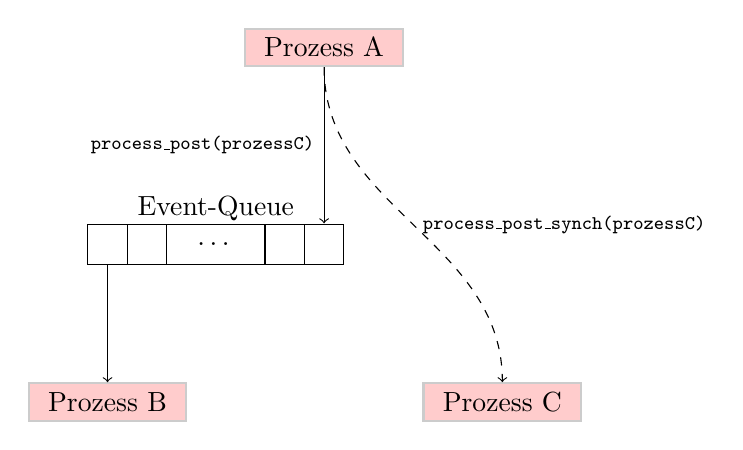
\begin{tikzpicture}
	\tikzstyle{aufruf}=[font=\ttfamily\scriptsize];
	\tikzstyle{funktion}=[draw,minimum width=2cm,fill=red!20,draw=black!20,thick];
	%\node (prozess) [funktion,below of=ph,below=1cm] {Prozess};


	\uncover<3->{
		\node [outer sep=0mm,inner sep=0mm] (eqout) at (0.25,0) {};
		\draw (0,0) -- (3.25,0) -- (3.25,.5) -- (0,.5) -- cycle;
		\draw (0.5,0) -- (0.5,0.5);
		\draw (1,0) -- (1,0.5);
		\node at(1.625,0.7) {Event-Queue};
		\node at (1.625,0.25) {\dots};
		\draw (2.25,0) -- (2.25,0.5);
		\draw (2.75,0) -- (2.75,0.5);
		\node [outer sep=0mm,inner sep=0mm] (eqin) at (3,.5) {};
	}
	\uncover<2->{\node (pa) [funktion,above of=eqin,above=1cm] {Prozess A};}
	\uncover<4->{\node (pb) [funktion,below of=eqout,below=.5cm] {Prozess B};}
	\uncover<5->{\node (pc) [funktion,right of=pb,right=3cm] {Prozess C};}

	\uncover<3->{\draw [->] (pa) -- node [aufruf,left] {process\_post(prozessC)} (eqin);}
	\uncover<4->{\draw [->] (eqout) -- (pb);}
	\uncover<5->{\draw [->] (pa) edge [in=90,out=270,dashed] node [aufruf,right] {process\_post\_synch(prozessC)} (pc);}
\end{tikzpicture}
